\documentclass[
  captions=tableheading,
  bibliography=totoc, 
  titepage=firstiscover,
]{scrartcl}

\usepackage{blindtext} %neuer input

\usepackage{longtable} % Tabellen über mehrere Seiten

\usepackage[utf8]{inputenc} %neuer input

\usepackage{scrhack}

\usepackage[aux]{rerunfilecheck} %Warnung falls nochmal kompiliert werden muss

\usepackage{fontspec} %Fonteinstellungen

\recalctypearea{}

\usepackage[main=ngerman]{babel} %deutsche Spracheinstellung

\usepackage{ragged2e} %neuer input

\usepackage{amsmath, nccmath}

\usepackage{amssymb} %viele mathe Symbole

\usepackage{mathtools} %Erweiterungen für amsmath


\DeclarePairedDelimiter{\abs}{\lvert}{\rvert}
\DeclarePairedDelimiter{\norm}{\lVert}{\rVert}

\DeclarePairedDelimiter{\bra}{\langle}{\rvert}
\DeclarePairedDelimiter{\ket}{\lvert}{\rangle}

\DeclarePairedDelimiterX{\braket}[2]{\langle}{\rangle}{
#1 \delimsize| #2
}

\NewDocumentCommand \dif {m}
{
\mathinner{\symup{d} #1}
}


\usepackage[
  math-style=ISO,
  bold-style=ISO,
  sans-style=italic,
  nabla=upright,
  partial=upright,
  warnings-off={
    mathtools-colon,
    mathtools-overbracket,
  },
]{unicode-math}

\setmathfont{Latin Modern Math}
\setmathfont{XITS Math}[range={scr, bfscr}]
\setmathfont{XITS Math}[range={cal, bfcal}, StylisticSet=1]


\usepackage[
  locale=DE,
  separate-uncertainty=true,
  per-mode=reciprocal,
  output-decimal-marker={,},
]{siunitx}

\usepackage[autostyle]{csquotes} %richtige Anführungszeichen

\usepackage{xfrac}

\usepackage{float}

\floatplacement{figure}{htbp}

\floatplacement{table}{htbp}

\usepackage[ %floats innerhalb einer section halten
  section,   %floats innerhalb er section halten
  below,     %unterhalb der Section aber auf der selben Seite ist ok
]{placeins}

\usepackage[
  labelfont=bf,
  font=small,
  width=0.9\textwidth,
]{caption}

\usepackage{subcaption} %subfigure, subtable, subref

\usepackage{graphicx}

\usepackage{grffile}

\usepackage{booktabs}

\usepackage{microtype} %Verbesserungen am Schriftbild

\usepackage[
backend=biber,
]{biblatex}

\addbibresource{../lit.bib}

\usepackage[ %Hyperlinks im Dokument
  german,
  unicode,
  pdfusetitle,
  pdfcreator={},
  pdfproducer={},
]{hyperref}

\usepackage{bookmark}

\usepackage[shortcuts]{extdash}

%\usepackage{warpcol}

\usepackage{tikz}

\newcommand*\circled[1]{\tikz[baseline=(char.base)]{
            \node[shape=circle,draw,inner sep=2pt] (char) {#1};}}

\begin{document}
    \title{V703: Das Geiger-Müller Zählrohr}
    \author{  
    Paul Störbrock\\
    \texorpdfstring{\href{mailto:paul.stoerbrock@tu-dortmund.de}{paul.stoerbrock@tu-dortmund.de}}{}
    }
    \date{Abgabe: 26.05.2020\vspace{-4ex}}
\maketitle
    
\newpage
\tableofcontents
\newpage

\setcounter{page}{1}

\section{Ziel}

\section{Theorie}

    \flushleft{Zu\;}\justifying

    \begin{figure}[H]
        \centering
        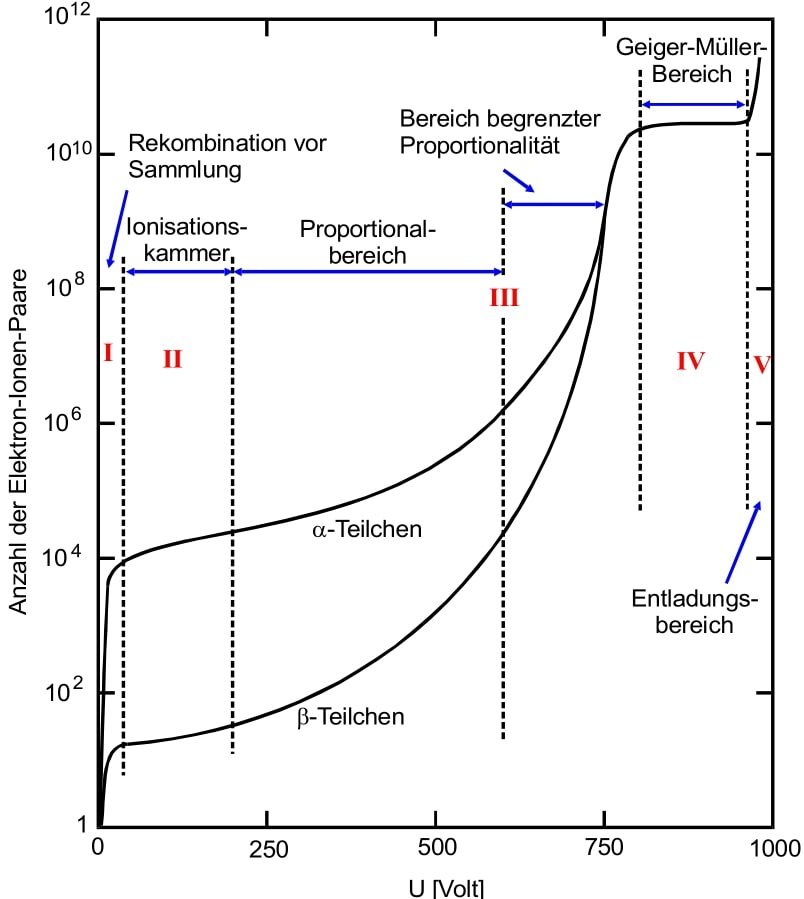
\includegraphics[width=\linewidth]{images/Messbereich.jpg}
        \caption{\cite{703}}
        \label{fig:1}
    \end{figure}

    \begin{figure}[H]
        \centering
        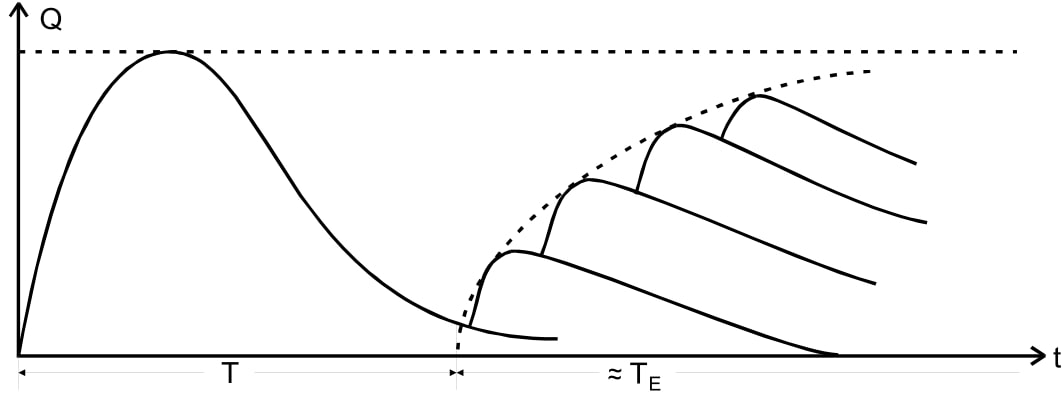
\includegraphics[width=\linewidth]{images/Erholungszeit.jpg}
        \caption{\cite{703}}
        \label{fig:2}
    \end{figure}

    \begin{figure}[H]
        \centering
        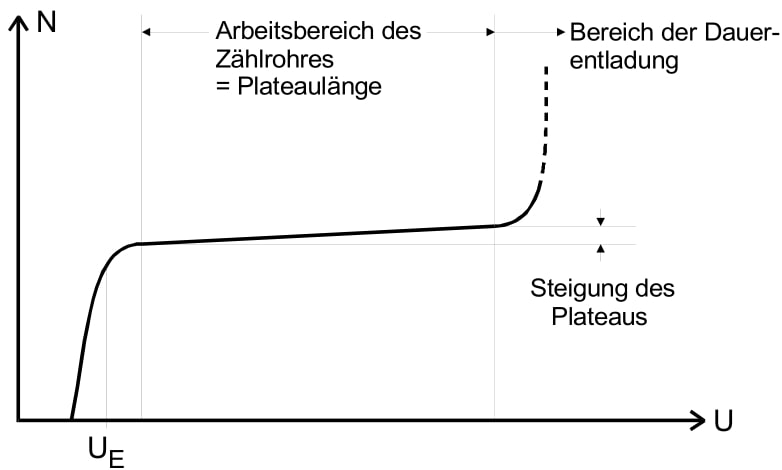
\includegraphics[width=\linewidth]{images/Plateau.jpg}
        \caption{\cite{703}}
        \label{fig:3}
    \end{figure}

\section{Versuchsaufbau und Durchführung}

    \flushleft{Zu\;}\justifying Beginn wird die Charakteristik des Zählrohrs gemessen, indem vor das Fenster des Zählrohrs eine $\beta$-Quelle,
    hier eine $^{204}$Tallium-Quelle, platziert und die Zählrate $N$ der Impulse in Abhängigkeit der Betriebsspannung $U$ gemessen wird. Dazu 
    wird der folgende Aufbau verwendet:

    \begin{figure}[H]
        \centering
        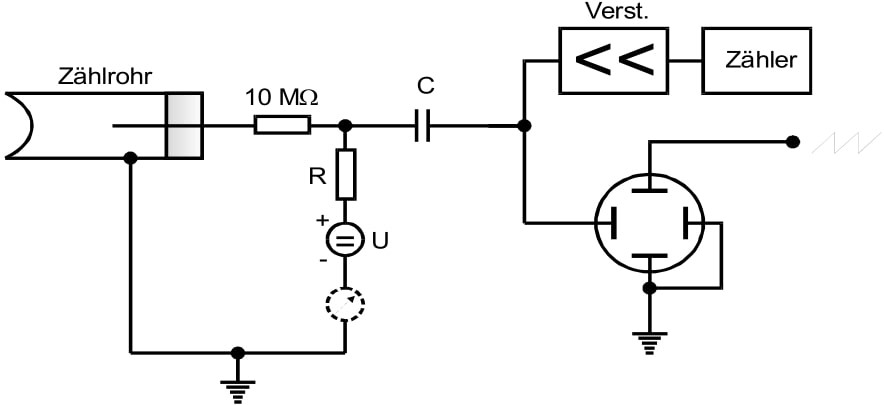
\includegraphics[width=\linewidth]{images/Aufbau.jpg}
        \caption{Aufbau des Geiger-Müller Zählrohrs samt Messaparatur \cite{703}}
        \label{fig:4}
    \end{figure}

    \flushleft{Dabei\;}\justifying sollte die maximale Impulsrate $\SI{100}{\per\second}$ Impulse nicht überschreiten. Die Impulsrate wird
    bei einer Startspannung von $\SI{320}{\volt}$ und fortlaufend in $\SI{10}{\volt}$-Schritten gemessen. Die Integrationszeit pro 
    Zählrohrspannung beträgt $\SI{60}{\second}$. Die Messungen werden bis zu einer Zählrohrspannung von $\SI{700}{\volt}$ durchgeführt. Dabei
    ist es wichtig zu beachten, dass die $\SI{700}{\volt}$ nicht überschritten werden dürfen, da das Zählrohr sonst zerstört werden würde.
    Neben der Impulsrate wird außerdem der Strom in $\SI{50}{\volt}$-Schritten dem Amperemeter entnommen.

    \flushleft{Um\;}\justifying die Totzeit des Geiger-Müller Zählrohrs zu erhalten, werden die Zwei-Quellen- und Oszilloskopmethode verwendet. 
    Für die Zwei-Quellen-Methode wird zuerst die $^{204}$Tallium-Quelle näher an das Geiger-Müller Zählrohr bewegt. Anschließend wird das zweite 
    Präparat hinzugestellt. Abschließend wird das erste Präparat entfernt. Für jeden der drei Schritte wird eine Integrationszeit von $\SI{120}
    {\second}$ verwendet. 

    \flushleft{Für\;}\justifying die Oszilloskopmethode wird die Zeit zwischen den ersten beiden Pulsen von dem folgenden Bild abgelesen:

    \begin{figure}[H]
        \centering
        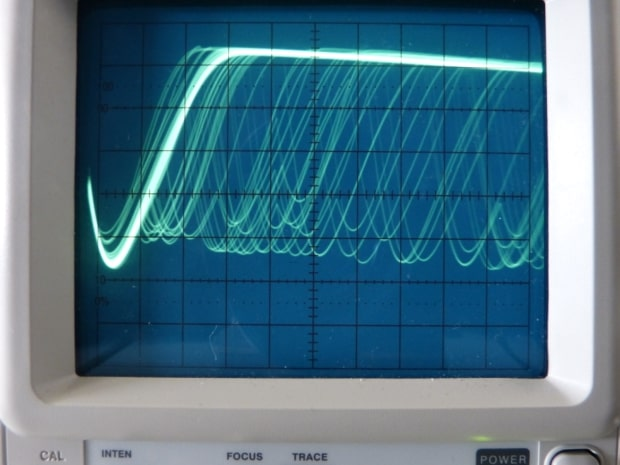
\includegraphics[width=\linewidth]{images/Oszilloskop.jpg}
        \caption{Momentaufnahme des Oszilloskops \cite{703}}
        \label{fig:5}
    \end{figure}

    \flushleft{Dabei\;}\justifying beträgt eine Kästchenlänge der Zeitachse $\SI{100}{\micro\second}$. 




\section{Auswertung}

\section{Diskussion}

\newpage
\printbibliography

\section{Appendix}

    \input{GM.tex}

    \begin{table}[H]
        \centering
        \input{strom.tex}
        \caption{Messwerte des Zählerstroms des Geiger-Müller Zählrohrs}
        \label{tab:1}
    \end{table}

\end{document}